\setModuleTitle{NGS Data \& FASTQ Format}
\setModuleAuthors{%
    Steve Pederson, Bioinformatics Hub, University of Adelaide \mailto{stephen.pederson@adelaide.edu.au}\\
}
\setModuleContributions{%
  Dan Kortschak, Adelson Research Group, University of Adelaide \mailto{dan.kortschak@adelaide.edu.au} \\
  Terry Bertozzi, SA Museum \mailto{Terry.Bertozzi@samuseum.sa.gov.au}
}

\chapter{\moduleTitle}
\newpage

\section{Initial Goals}

\begin{enumerate}
\item Understand the \textit{Sequencing by Synthesis} Process \& Data Generation \\
\item Understand what errors and artefacts lie within the data \\
\item Learn how to assess the quality of data \& make informed decisions \\
\end{enumerate}

\section{NGS Data Generation}
\begin{steps}
Before we can begin to analyse any data, it is helpful to understand how it was generated.
Whilst there are numerous platforms for generation of NGS data, today we will look at the Illumina \textit{Sequencing by Synthesis} method, which is one of the most common methods in use today.
Many of you will be familiar with the process involved, but it may be worth looking at the following 5-minute video from Illumina: \url{http://youtu.be/womKfikWlxM} 
%As setting up the sound with the VMs can be tricky, it will be easier to view this from your own regular browser.
%Briefly minimise the VM (see Section 1.4), open your regular browser \& please use your headphones if you brought them. \\
\end{steps}

\begin{note}
This video refers to the process \textit{tagmentation}.
This is a relatively recent method for fragmenting \& attaching adaptors to DNA, with an alternative, more traditional method being sonication, poly-adenylation \& attachment of appropriate adaptors in separate steps.
The important concept to note during sample preparation is that the DNA insert has multiple sequences ligated to either end.
These include 1) the \textit{sequencing primers}, 2) index or \textit{barcode} sequences, and 3) the flow-cell binding oligos.
\end{note}

\begin{questions}
Assuming each 'spot' on the flowcell is generated from a unique DNA sequence, there are two important sequencing errors that will occur during this process.
What do you think they might be? \\
\begin{answer}
1) Ligation of the wrong base during sequencing \\
2) Insertions \& deletions \\
It's the same basic errors as normal DNA replication, but without the \textit{in vivo} DNA repair mechanisms.
\end{answer}

Will these errors have a more significant effect if they occur during the sequence detection stage, or during generation of the DNA clones within each cluster? \\
\begin{answer}
The earlier in the process any sequencing errors occur, the higher the degree to which they will be propagated.
If an error occurs during the very first round of amplification, before even bridge amplification, it will be propagated through an entire cluster. \\
\end{answer}

Will all of the individual ssDNA molecules within a spot be amplified perfectly in sync with each other?\\
\begin{answer}
No.  As the reads become longer, the more molecules will get out of sync (i.e. phase) with each other.
As a result the quality scores will drop off towards the end of a read.
\end{answer}
\end{questions}

\section{Today's Data}
\begin{steps}
The raw data for today's workshop needs to be downloaded and placed in the directory \texttt{/home/trainee/NGSData}.
First we'll have to change into our home directory and create this new sub-directory
\begin{lstlisting}
cd
mkdir NGSData
\end{lstlisting}

There are four main datasets we'll look at today and we'll download them all as we need them.
The first dataset today is some RNA-Seq reads, so let's create a directory to place the data in
\begin{lstlisting}
cd ~/NGSData
mkdir -p RNASeq/rawData
\end{lstlisting}
\end{steps}

\begin{questions}
What did the \texttt{-p} option do in the previous line?\\
\begin{answer}
Enabled building any missing parent directories.
\end{answer}
This was a quick \& dirty shortcut.
Why might this be a bad idea?\\
\begin{answer}
Being cautious ensures we set the correct structure in the correct place, without typos.\\
\end{answer}
\end{questions}

\begin{steps}
Now we have somewhere to put our data, let's download it.
This is probably the best time to use cut \& paste from the electronic copy of these notes.
When in the \texttt{bash shell} we can copy using \texttt{Ctrl + Shift + V} and we can paste using \texttt{Ctrl + Shift + V}.
Also note that for the second line, you can use the up arrow and just change the end of the line from \texttt{reads1.fq.gz} to \texttt{reads2.fq.gz}.

\begin{lstlisting}
wget https://swift.rc.nectar.org.au:8888/v1/AUTH_33065ff5c34a4652aa2fefb292b3195a/IntroNGS_2014/reads1.fq.gz
wget https://swift.rc.nectar.org.au:8888/v1/AUTH_33065ff5c34a4652aa2fefb292b3195a/IntroNGS_2014/reads2.fq.gz
\end{lstlisting}

\end{steps}

\section{FASTQ File Format}
\begin{note}
As the sequences are extended during the sequencing reaction, an image is recorded which is effectively a movie or series of frames at which the addition of bases is recorded \& detected.
We mostly don't deal with these image files, but will handle data generated from these in \textit{fastq} format, which can commonly have the file suffix \textit{.fq} or \textit{.fastq}.
As these files are often very large, they will often be zipped using \texttt{gzip} or \texttt{bzip}.
Whilst we would instinctively want to unzip these files using the command \texttt{gunzip}, most NGS tools are able to work with zipped fastq files, and this is usually unnecessary.
This can save considerable hard drive space, which is an important consideration when handling NGS datasets as the quantity of data can easily push your storage capacity to it's limit. \\
\end{note}

\begin{steps}
We should still have a terminal open from the previous section \&, if necessary, use the \texttt{cd} command to make sure you are in the \texttt{\~{}/NGSData/RNASeq/rawData} directory.
The command \texttt{zcat} unzips a file \& prints the output to the terminal, or standard output (\textit{stdout}).
If we did this to these files, we would see a stream of data whizzing past in the terminal, but instead we can just pipe the output of \texttt{zcat} to the command head to view the first 10 lines of a file. \\
\begin{lstlisting}
cd ~/NGSData/RNASeq/rawData
zcat reads1.fq.gz | head -n8
\end{lstlisting}
\end{steps}

\begin{information}
In the above command, we have used a trick commonly used in Linux systems where we have taken the output of one command (\texttt{zcat reads1.fq.gz}) and sent it to another command (\texttt{head}) by using the \textit{pipe symbol} (|).
This is literally like sticking a pipe on the end of a process \& redirecting the output to the input another process.
If you think of things as being like a data factory you can almost visualise it.
There are no limits to the number of commands that you can string together using this trick. 
Additionally, we gave the argument \texttt{-n8} to the command \texttt{head} to ensure that we only printed the first eight lines.\\
\end{information}

\begin{warning}
\large{Don't Panic!!!} \\
\normalsize
If at some stage today you find that the terminal has become unresponsive, or you are seeing an unexpected stream of data fly past, you can abort whichever process is currently running in the terminal by entering \texttt{Ctrl-c}.
This is an instruction to the computer to `kill the current process.' \& you may be surprised at how often this comes in handy.
Even experienced programmers rely on this trick from time to time.
\end{warning}

\begin{note}
In the output from the above terminal command, we have obtained the first 8 lines of the gzipped fastq file.
This gives a clear view of the fastq file format, where each individual read spans four lines.
These lines are:
\begin{enumerate}
\item The read identifier
\item The sequence read
\item An alternate line for the identifier (commonly left blank as just a \texttt{+} symbol acting as a placeholder)
\item The quality scores for each position along the read as a series of ascii text characters.
\end{enumerate}
\end{note}

Let's have a brief look at each of these lines and what they mean.\\

\subsubsection*{The read identifier}
This line begins with an \texttt{@} symbol and although there is some variability, it traditionally has several components.
Today's data have been sourced from an EBI data repository with the identifier \texttt{SRR031714}.
For the first sequence in this file, we have the full identifier \texttt{@SRR031714.1 HWI-EAS299\_130MNEAAXX:2:1:785:591/1} which has the following components: \\

\begin{tabular}{|p{5cm} | p{9cm} |}
  \hline
  \texttt{SRR031714.1} & The aforementioned EBI identifier \& the sequence ID within the file. As this is the first read, we have the number 1. NB: This identifier is \textbf{not} present when data is obtained directly from the machine or service provider.\\
  \hline
  \texttt{WHI-EAS299\_130MNEAAXX} & The unique machine ID \\
  \hline
  \texttt{2} & The flowcell lane \\
  \hline
  \texttt{1} & The tile within the flowcell lane \\
  \hline
  \texttt{785} & The $x$-coordinate of the cluster within the tile \\
  \hline
  \texttt{591} & The $y$-coordinate of the cluster within the tile \\
  \hline
  \texttt{/1} & Indicates that this is the first read in a set of paired end reads \\
  \hline
\end{tabular}

As seen in the subsequent sections, these pieces of information can be helpful in identifying if any spatial effects have affected the quality of the reads.
By and large you won't need to utilise most of this information, but it can be handy for times of serious data exploration.\\

\begin{steps}
While we are inspecting our data, have a look at the beginning of the second file.
\begin{lstlisting}
zcat reads2.fq.gz | head -n8
\end{lstlisting}
Here you will notice that the information in the identifier is identical to the first file we inspected, with the exception that there is a \texttt{/2} at the end.
This indicates that these reads are the second set in what are known as \textit{paired-end} reads, as were introduced in the above video.
The two files will have this identical structure where the order of the sequences in one is identical to the order of the sequences in the other.
This way when they are read as a pair of files, they can be stepped through read-by-read \& the integrity of the data will be kept intact.
\end{steps}

\subsubsection{The Illumina Chastity Filter}
\begin{information}
It is also worth noting that the reads we've just glanced at come from a version of the Illumina \textit{casava} pipeline which is \textless 1.8, and which is a relatively common format.
The casava version really just describes how old the software on the Illumina machine is \& we don't choose this.
For more recently generated reads where the casava software is \textgreater 1.8 of the casava, there is an additional field in the identifier which indicates whether a read would have \textit{failed} an initial QC check. 
An example of this format would be:
\begin{lstlisting}
@D5B4KKQ1:554:C4YHPACXX:4:1101:1084:2100 1:Y:0:
\end{lstlisting}
Note the ``Y'' in the final fields, which indicates this sequence would have \textbf{failed} QC.
These low-quality reads were automatically removed in earlier versions of the pipeline and were omitted from the fastq file.
However, they are now included with this additional field indicated in the read identifier.
Inspection of this line will enable you to find out which version of the casava pipeline has been used, and whether you need to perform any additional filtering steps to remove low quality reads. 
The tool \texttt{fastq\_illumina\_filter} is designed to remove these reads for you \& the tool, along with usage instructions can be found at \url{http://cancan.cshl.edu/labmembers/gordon/fastq\_illumina\_filter/}.\\
\end{information}

\begin{steps}
An alternate set of reads which we'll also explore today is in included in the directory \texttt{\~{}/NGSData/iCLIP/rawData}.
These are immunopreciptated mRNAs and were supplied by some collaborators who'd either forgotten the removal of low-quality reads or had deliberately neglected step to increase read numbers.
Note that these files are not compressed and are essentially plain text files, so we can directly inspect them using the command \texttt{head} instead of decompressing first.\\
\end{steps}

\begin{lstlisting}
cd ~/NGSData/iCLIP/rawData
head -n12 iCLIP_Sample1.fastq
\end{lstlisting}

Note that the header lines follow the format described on the previous page with this additional field at the end of the line.
\begin{questions}
Of the first three reads which have been printed to the terminal above, which one(s) will have failed the chastity filter, and which ones will have passed the filter?\\
\begin{answer}
The first read would have failed (i.e. it is low quality), whilst the other two will have passed.
\end{answer}
\end{questions}

\subsubsection{Quality Scores}
\begin{information}
The only other line in the fastq format that really needs some introduction is the quality score information.
These are presented as single \textit{ascii} text characters for simple visual alignment with the sequence, and each character corresponds to a numeric value, which is the quality score.
In the ascii text system, each character has a numeric value which we can interpret as an integer.
Head to the website with a description of these at \url{http://en.wikipedia.org/wiki/ASCII#ASCII\_printable\_code\_chart}.\\

The first 31 characters are non-printable \& contain things like end-of-line marks and tab spacings, and note that the first printable character after the space is `!' which corresponds to the value 33.
In short, the values 33-47 are symbols like !, \", \#, \$ etc, whereas the values 48-57 are the characters 0-9.
Next are some more symbols (including @ for the value 64), with the upper case characters representing the values 65-90 \& the lower case letters representing the values 97-122.\\

In the line of quality scores for the first read in the iCLIP sample above, the first character is ``=", so this base has a quality score of 61.
The second symbol in this line is``D", so the second base has a quality score of 68.
\end{information}

\subsubsection{The PHRED +33/64 Scoring System}
\begin{information}
Now that we understand how to turn the quality scores from an ascii character into a numeric value, we need to know what these numbers represent.
The two main systems in common usage are PHRED +33 and PHRED +64 and for each of these coding systems we either subtract 33 or 64 from the numeric value associated with each ascii character to give us a PHRED score.
As will be discussed later, this score ranges between 0 and about 41.\\

The PHRED system used is determined by the software installed on the sequencing machine, with early machines using PHRED + 64 (casava \textless 1.5), and more recent machines tending to use PHRED + 33.
For example, in PHRED +33, the @ symbol corresponds to Q = 64 - 33 = 31, whereas in PHRED +64 it corresponds to Q = 64 - 64 = 0. \\
\end{information}

\begin{minipage}{\textwidth}

The following table demonstrates the comparative coding scale for the different formats: \\

\scriptsize
\texttt{...............................IIIIIIIIIIIIIIIIIIIIIIIIIIIIIIIIIIIIIIIII...................... \\
.................................\textbf{J}JJJJJJJJJJJJJJJJJJJJJJJJJJJJJJJJJJJJJJ...................... \\
LLLLLLLLLLLLLLLLLLLLLLLLLLLLLLLLLLLLLLLLLL.................................................... \\
!"\#\$\%\&'()*+,-./0123456789:;\textless =\textgreater?@ABCDEFGHIJKLMNOPQRSTUVWXYZ[\textbackslash]\^{}\_`abcdefghijklmnopqrstuvwxyz\{|\}\~{}} \\
\texttt{
~~|~~~~~~~~~~~~~~~~~~~~~~~~~|~~~~|~~~~~~~~|~~~~~~~~~~~~~~~~~~~~~~~~~~~~~~|~~~~~~~~~~~~~~~~~~~~~|~\\
~33~~~~~~~~~~~~~~~~~~~~~~~~59~~~64~~~~~~~73~~~~~~~~~~~~~~~~~~~~~~~~~~~~104~~~~~~~~~~~~~~~~~~~126~\\
~ \\
I - Illumina 1.3+ Phred+64,  raw reads typically (0, 40) \\ 
J - Illumina 1.5+ Phred+64,  raw reads typically (3, 40) \\
L - Illumina 1.8+ Phred+33,  raw reads typically (0, 41) \\
}
%\normalsize
\end{minipage}

\begin{questions}
Have a look at the quality scores in the RNA-Seq data. 
Which coding system do you think has been used for the RNA-Seq reads that we have? \\
\begin{answer}
PHRED+33. 
The presence of values between `!' \& `?' gives this away.\\
\end{answer}
In the PHRED +33 coding system, the character `@' is used.
Can you think of any potential issues this would cause when searching within a fastq file? 
(Hint: Consider the sequence identifier rows)\\
\begin{answer}
It is also included as the beginning of each sequence identifier.
If located at the beginning of a string of quality scores, this may be misunderstood as a sequence identifier.
This is good to keep in mind when writing custom code for searching fastq files.
\end{answer}
\end{questions}

\subsubsection{Interpretation of PHRED Scores}

\begin{information}
All NGS platforms have non-zero error rates during the sequencing process (\url{http://www.molecularecologist.com/next-gen-table-3c-2014/}), and the quality scores are related to the probability of calling an incorrect base.
The PHRED scoring system predates NGS technologies \& is based on whether the wavelength from one specific base is clearly dominant through the formula
\begin{equation}
  \label{eq:PHRED}
  Q = -10 log_{10} P
\end{equation}
where $P$ is the probability of calling the incorrect base. \\
\end{information}

This is more easily seen in the following table: \\
\begin{center}
\begin{tabular}[h]{|p{3cm} p{5cm} p{3cm}|}
\hline
\textbf{PHRED Score} & \textbf{Probability of Incorrect Base Call} &
\textbf{Accuracy of Base Call} \\
\hline
0 & 1 in 1 & 0\% \\
10 & 1 in 10 & 90\% \\
20 & 1 in 100 & 99\% \\
30 & 1 in 1000 & 99.9\% \\
40 & 1 in 10000 & 99.99\% \\
\hline
\end{tabular}
\end{center}

\begin{note}
As each base is added, the light wavelength associated with each base (i.e. the colour) is detected.
In theory, there should only be one colour observed, but in reality there will always be a residual signal from the other bases.
The following chromatogram based on the traditional Sanger sequencing methods demonstrates this well (Source: \url{http://seqcore.brcf.med.umich.edu}.\\
\end{note}

\begin{figure}[h!]
  \centering
    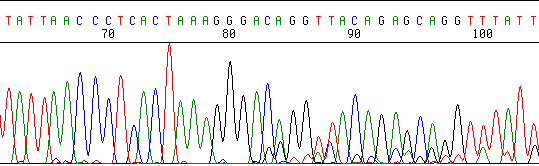
\includegraphics[width=0.8\textwidth]{clonesite.png}
\end{figure}

Note that early in this sequence, the colour peaks are clear but with small residual peaks of background signal.
These peaks would receive high PHRED scores.
Around position 83 however, the peaks become less obvious and any corresponding PHRED score would be lower.
This basic principle is applied on a massively parallel scale during the generation of NGS data.\\

\begin{questions}
A common threshold for inclusion of a sequence is that all bases must have a Q score $>20$.
Considering the millions of sequences obtained from a flowcell, do you think that NGS data is likely to be highly accurate?\\
\begin{answer}
This is really just a point for everyone to ponder.
People should be encouraged to realise that NGS data will have a lot of errors...
\end{answer}
\end{questions}

\clearpage
